% Options for packages loaded elsewhere
\PassOptionsToPackage{unicode}{hyperref}
\PassOptionsToPackage{hyphens}{url}
\PassOptionsToPackage{dvipsnames,svgnames,x11names}{xcolor}
%
\documentclass[
  9pt,
  twocolumn,
  twoside]{pnas-new}

\usepackage{amsmath,amssymb}
\usepackage{iftex}
\ifPDFTeX
  \usepackage[T1]{fontenc}
  \usepackage[utf8]{inputenc}
  \usepackage{textcomp} % provide euro and other symbols
\else % if luatex or xetex
  \usepackage{unicode-math}
  \defaultfontfeatures{Scale=MatchLowercase}
  \defaultfontfeatures[\rmfamily]{Ligatures=TeX,Scale=1}
\fi
\usepackage{lmodern}
\ifPDFTeX\else  
    % xetex/luatex font selection
\fi
% Use upquote if available, for straight quotes in verbatim environments
\IfFileExists{upquote.sty}{\usepackage{upquote}}{}
\IfFileExists{microtype.sty}{% use microtype if available
  \usepackage[]{microtype}
  \UseMicrotypeSet[protrusion]{basicmath} % disable protrusion for tt fonts
}{}
\makeatletter
\@ifundefined{KOMAClassName}{% if non-KOMA class
  \IfFileExists{parskip.sty}{%
    \usepackage{parskip}
  }{% else
    \setlength{\parindent}{0pt}
    \setlength{\parskip}{6pt plus 2pt minus 1pt}}
}{% if KOMA class
  \KOMAoptions{parskip=half}}
\makeatother
\usepackage{xcolor}
\setlength{\emergencystretch}{3em} % prevent overfull lines
\setcounter{secnumdepth}{-\maxdimen} % remove section numbering
% Make \paragraph and \subparagraph free-standing
\ifx\paragraph\undefined\else
  \let\oldparagraph\paragraph
  \renewcommand{\paragraph}[1]{\oldparagraph{#1}\mbox{}}
\fi
\ifx\subparagraph\undefined\else
  \let\oldsubparagraph\subparagraph
  \renewcommand{\subparagraph}[1]{\oldsubparagraph{#1}\mbox{}}
\fi


\providecommand{\tightlist}{%
  \setlength{\itemsep}{0pt}\setlength{\parskip}{0pt}}\usepackage{longtable,booktabs,array}
\usepackage{calc} % for calculating minipage widths
% Correct order of tables after \paragraph or \subparagraph
\usepackage{etoolbox}
\makeatletter
\patchcmd\longtable{\par}{\if@noskipsec\mbox{}\fi\par}{}{}
\makeatother
% Allow footnotes in longtable head/foot
\IfFileExists{footnotehyper.sty}{\usepackage{footnotehyper}}{\usepackage{footnote}}
\makesavenoteenv{longtable}
\usepackage{graphicx}
\makeatletter
\def\maxwidth{\ifdim\Gin@nat@width>\linewidth\linewidth\else\Gin@nat@width\fi}
\def\maxheight{\ifdim\Gin@nat@height>\textheight\textheight\else\Gin@nat@height\fi}
\makeatother
% Scale images if necessary, so that they will not overflow the page
% margins by default, and it is still possible to overwrite the defaults
% using explicit options in \includegraphics[width, height, ...]{}
\setkeys{Gin}{width=\maxwidth,height=\maxheight,keepaspectratio}
% Set default figure placement to htbp
\makeatletter
\def\fps@figure{htbp}
\makeatother
% definitions for citeproc citations
\NewDocumentCommand\citeproctext{}{}
\NewDocumentCommand\citeproc{mm}{%
  \begingroup\def\citeproctext{#2}\cite{#1}\endgroup}
\makeatletter
 % allow citations to break across lines
 \let\@cite@ofmt\@firstofone
 % avoid brackets around text for \cite:
 \def\@biblabel#1{}
 \def\@cite#1#2{{#1\if@tempswa , #2\fi}}
\makeatother
\newlength{\cslhangindent}
\setlength{\cslhangindent}{1.5em}
\newlength{\csllabelwidth}
\setlength{\csllabelwidth}{3em}
\newenvironment{CSLReferences}[2] % #1 hanging-indent, #2 entry-spacing
 {\begin{list}{}{%
  \setlength{\itemindent}{0pt}
  \setlength{\leftmargin}{0pt}
  \setlength{\parsep}{0pt}
  % turn on hanging indent if param 1 is 1
  \ifodd #1
   \setlength{\leftmargin}{\cslhangindent}
   \setlength{\itemindent}{-1\cslhangindent}
  \fi
  % set entry spacing
  \setlength{\itemsep}{#2\baselineskip}}}
 {\end{list}}
\usepackage{calc}
\newcommand{\CSLBlock}[1]{\hfill\break\parbox[t]{\linewidth}{\strut\ignorespaces#1\strut}}
\newcommand{\CSLLeftMargin}[1]{\parbox[t]{\csllabelwidth}{\strut#1\strut}}
\newcommand{\CSLRightInline}[1]{\parbox[t]{\linewidth - \csllabelwidth}{\strut#1\strut}}
\newcommand{\CSLIndent}[1]{\hspace{\cslhangindent}#1}

% TODO: Add custom LaTeX header directives here
\makeatletter
\@ifpackageloaded{caption}{}{\usepackage{caption}}
\AtBeginDocument{%
\ifdefined\contentsname
  \renewcommand*\contentsname{Table of contents}
\else
  \newcommand\contentsname{Table of contents}
\fi
\ifdefined\listfigurename
  \renewcommand*\listfigurename{List of Figures}
\else
  \newcommand\listfigurename{List of Figures}
\fi
\ifdefined\listtablename
  \renewcommand*\listtablename{List of Tables}
\else
  \newcommand\listtablename{List of Tables}
\fi
\ifdefined\figurename
  \renewcommand*\figurename{Figure}
\else
  \newcommand\figurename{Figure}
\fi
\ifdefined\tablename
  \renewcommand*\tablename{Table}
\else
  \newcommand\tablename{Table}
\fi
}
\@ifpackageloaded{float}{}{\usepackage{float}}
\floatstyle{ruled}
\@ifundefined{c@chapter}{\newfloat{codelisting}{h}{lop}}{\newfloat{codelisting}{h}{lop}[chapter]}
\floatname{codelisting}{Listing}
\newcommand*\listoflistings{\listof{codelisting}{List of Listings}}
\makeatother
\makeatletter
\makeatother
\makeatletter
\@ifpackageloaded{caption}{}{\usepackage{caption}}
\@ifpackageloaded{subcaption}{}{\usepackage{subcaption}}
\makeatother
\ifLuaTeX
  \usepackage{selnolig}  % disable illegal ligatures
\fi
\usepackage{bookmark}

\IfFileExists{xurl.sty}{\usepackage{xurl}}{} % add URL line breaks if available
\urlstyle{same} % disable monospaced font for URLs
\hypersetup{
  pdftitle={Mapping Mixtures of Genotype-by-Weather Interactions in Switchgrass (Panicum virgatum)},
  pdfauthor={Alice H. MacQueen; Li Zhang; Samuel A. Smith; Jason Bonnette; Arvid R. Boe; Phillip A. Fay; Felix B. Fritschi; David B. Lowry; Robert B. Mitchell; Francis M. Rouquette Jr; Yanqi Wu; Arbel Harpak; Thomas E. Juenger},
  pdfkeywords={allele-by-environment effect variation, antagonistic
pleiotropy, photoperiod, cumulative rainfall, genetic variation},
  colorlinks=true,
  linkcolor={blue},
  filecolor={Maroon},
  citecolor={Blue},
  urlcolor={Blue},
  pdfcreator={LaTeX via pandoc}}

\templatetype{pnasresearcharticle}

\title{Mapping Mixtures of Genotype-by-Weather Interactions in
Switchgrass (Panicum virgatum)}

\newcommand{\equalcont}{1}

\newcommand{\correspond}{2}

\author[a%
,\equalcont%
,\correspond%
]{Alice H. MacQueen}
\author[a%
,\equalcont%
%
]{Li Zhang}
\author[a%
,\equalcont%
%
]{Samuel A. Smith}
\author[a%
%
%
]{Jason Bonnette}
\author[b%
%
%
]{Arvid R. Boe}
\author[c%
%
%
]{Phillip A. Fay}
\author[d%
%
%
]{Felix B. Fritschi}
\author[e%
%
%
]{David B. Lowry}
\author[f%
%
%
]{Robert B. Mitchell}
\author[g%
%
%
]{Francis M. Rouquette Jr}
\author[h%
%
%
]{Yanqi Wu}
\author[a%
%
%
]{Arbel Harpak}
\author[a%
%
,\correspond%
]{Thomas E. Juenger}

\affil[a]{University of Texas at Austin, Department of Integrative
Biology, Austin, 78712}
\affil[b]{South Dakota State University, Department of
Agronomy, Brookings, 57006}
\affil[c]{USDA-ARS, Grassland, Soil and Water Research
Laboratory, Temple, 76502}
\affil[d]{University of Missouri, Division of Plant
Sciences, Columbia, 65211}
\affil[e]{Michigan State University, Department of Plant Biology, East
Lansing, 48824}
\affil[f]{USDA-ARS, Wheat, Sorghum, and Forage Research
Unit, Lincoln, 68583}
\affil[g]{Texas A\&M University, Texas A\&M AgriLife Research and
Extension Center, Overton, 75684}
\affil[h]{Oklahoma State University, Department of Plant and Soil
Sciences, Stillwater, 74078}

\leadauthor{MacQueen}

\significancestatement{The timing of plant seasonal development
(phenology) has major impacts on fitness because of the steep fitness
cost of plant-environment mismatches. We infer the mixture of ways that
genetic effects on phenological traits depend on plant environment,
focusing on how effects covary with weather prior to the phenological
event (GxWeather). Most effects do not have GxWeather, but a minority
do. GxWeather is population-specific. The majority of effects on the
timing of vegetative growth in the Gulf population have GxWeather: these
effects differ in sign across environments and covary with a photoperiod
cue two weeks prior. A minority of effects on flowering date in the Gulf
and Midwest populations had GxWeather, covarying with a cumulative
rainfall and a photoperiod cue, respectively.}

\authorcontributions{T.E.J. designed research. D.B.L. contributed plant
material and resources. J.B., D.B.L., and T.E.J. designed and executed
field experiments. A.R.B., P.A.F., F.B.F., D.B.L., R.B.M., F.M.R., Y.W.,
and T.E.J. hosted field experiments. A.H.M., L.Z., and S.A.S. conducted
statistical and computational analyses. The manuscript was written by
A.H.M. with contributions from all authors.}

\authordeclaration{The authors declare no conflicts of interest.}

\equalauthors{\textsuperscript{\equalcont} A.H.M. contributed equally to
this work with L.Z. and S.A.S.}

\correspondingauthor{\textsuperscript{\correspond}To whom correspondence should be addressed. E-mail: alicem@uchicago.edu}
\correspondingauthor{\textsuperscript{\correspond}To whom correspondence should be addressed. E-mail: tjuenger@utexas.edu}

\keywords{allele-by-environment effect variation | antagonistic
pleiotropy | photoperiod | cumulative rainfall | genetic variation}

\begin{document}
\maketitle

\begin{abstract}
The timing of vegetative and reproductive growth in plants
(``phenological timings'') depends on both genetic variation and
environmental cues; thus, phenological traits can have important
genotype-by-environment (GxE) interactions. Identifying the mixture and
prevalence of GxE primed by weather prior to the phenological event
(GxWeather) should aid prediction and manipulation of phenological
timings. Here, we map GxWeather effects on phenological timings in two
highly divergent switchgrass (\emph{Panicum virgatum}) populations using
repeated plantings of cloned individuals from these populations at eight
sites spanning the central United States. We distinguish GxWeather
patterns covarying with interpretable weather-based cues from agnostic,
site-based patterns. Most GxWeather effects belong to the latter
category and do not covary with weather-based cues. However, 65\% of
effects on the timing of vegetative growth in the Gulf population covary
with daylength 14 days prior to green-up date. 33\% of effects on the
timing of flowering in the Gulf population covary with cumulative
rainfall in the seven days prior to flowering, while 22\% of effects on
flowering timing in the Midwest population covary with day length change
two days prior to flowering. An independent pseudo-F2 cross of Gulf and
Midwest individuals at the same sites mapped 10 additive QTLs for
flowering and three for vegetative growth timing, all with significant
associations and three with enrichment of highly significant
associations in our model of GxWeather effects. We demonstrate that we
can identify genetic variation with GxWeather and assign these loci to
specific weather-based cues or other patterns. Breeding for particular
alleles at these loci could change flowering responsiveness to
photoperiod and rainfall cues in switchgrass. More broadly, this
approach could be used to identify genetic marker-environment
interactions in any species with related populations phenotyped in
multiple environments.
\end{abstract}

\dates{This manuscript was compiled on \today}
\doi{\url{www.pnas.org/cgi/doi/10.1073/pnas.XXXXXXXXXX}}

\thispagestyle{firststyle}
\ifthenelse{\boolean{shortarticle}}{\ifthenelse{\boolean{singlecolumn}}{\abscontentformatted}{\abscontent}}{}
\firstpage[8]{2}

Plant phenological timings are major components of plant fitness
affected by multiple external environmental cues (e.g.~degree of winter
chilling, day length, temperature, and water availability) that signal
existing or upcoming growing conditions (1--3). Genetic responses to
environmental cues determine the speed, timing, and energy apportioned
to vegetative and reproductive growth and shape both the individual's
lifespan and its lifetime production of viable seed. Day length (or
photoperiod) is one of the most predictable environmental cues, and
genetic sensitivity to photoperiod protects plants from potentially
fatal consequences of phenological responses to temperature cues at the
``wrong'' time of year. However, the usefulness of specific
environmental cues depends on both features of the environment, such as
cue predictability and relevance, and the species' adaptive strategies
(4). Species with wide natural distributions can have multiple distinct
environmentally cued phenological responses: for example, populations of
sunflower (\emph{Helianthus annuus}) exhibit day-neutral, facultative
short day, and facultative long-day flowering responses, which vary with
their environments (5, 6). Distinct genetic responses in different
environments are known as genotype by environment interactions, or GxE.

Flowering time, or the transition from vegetative to reproductive
growth, is a common subject of GxE research (5--11), a key output of
selection driving adaptation to local environments (2, 12, 13), and a
selection target for crop improvement to adapt crops to local or future
environments (14). Changing flowering responsiveness to photoperiod cues
has allowed geographic range expansion and increased yields in several
cereal species (15--19) and other crops (20, 21). Recent statistical
advances in studying phenological GxE have involved determining critical
environmental indices before the phenological event occurs, such as
photothermal time within a critical growth window (10). However, most
studies of flowering GxE focus on finding a single, best fitting form of
genotype-environment covariance, despite the key expectation that
different genetic subpopulations, and even different genomic regions,
have likely evolved distinct patterns of GxE. Additionally, despite
theoretical predictions that local adaptation should involve
antagonistic pleiotropy, or sign-changing GxE, at the level of
individual loci (22--25), previous work has found limited evidence of
antagonistic pleiotropy (12, 26). However, this work has been limited by
a known statistical bias that reduced detection of genetic effects that
differ in sign (26--28). Thus, despite substantial interest in the
frequencies of various forms of GxE, the prevalence of antagonistic
pleiotropy relative to other forms of GxE remains unknown.

Previous research suggests that switchgrass phenological timings should
have GxWeather and that these timings could differ by genetic
subpopulation. Switchgrass is considered a short-day plant with
reproductive development strongly linked to day of the year (29).
However, as part of its wide environmental adaptation across the eastern
half of North America, its photoperiodicity has been predicted to differ
by plant latitude of origin (30, 31). We previously found divergent
Midwest and Gulf genetic subpopulations of switchgrass with distinct
sets of environmental adaptations, in that both populations had distinct
genetic variation associated with each of two fitness proxies, biomass
and survival (32). The Midwest genetic subpopulation is primarily
composed of individuals from the well-studied upland switchgrass ecotype
(33, 34), while the Gulf subpopulation has individuals from the
well-studied lowland ecotype and the phenotypically intermediate coastal
ecotype (32).

Here, we estimate GxWeather for two phenological timings in switchgrass
by assigning patterns of genetic effects on phenology across gardens to
many patterns of weather covariance at these gardens. To do this, we
phenotype a diversity panel of hundreds of switchgrass genotypes from
the Midwest and Gulf subpopulations for the timing of vegetative and
reproductive development at eight common garden locations spanning 17
degrees of latitude. These gardens cover the majority of the latitudinal
and climatic range of switchgrass and capture the most comprehensive
picture to date of the environmental variation this species encounters.
We define multiple ways phenological timings might covary with weather
(@tbl-covar) and additional ways phenological timings might vary by site
(@SI-info), then jointly re-estimate genetic effects on these timings at
all eight sites using the set of these covariance matrices that
significantly improved the modeled log-likelihood when included
(@SI-info) (35). We use the Bayesian framework \emph{mash} (multivariate
adaptive shrinkage), developed by (35), to refine effect size estimates
from genome-wide association (GWAS) conducted on individuals at each of
the eight sites. \emph{mash} allows us to identify and specify multiple
covariance structures among genetic effect estimates across sites,
including structures that represent covariance in weather variables of
interest. Importantly, \emph{mash} does not have a statistical bias in
detecting genetic effects with the same or opposite signs (36). To
confirm our genetic mapping of GxWeather, we compare our posterior
genetic effect estimates from \emph{mash} to mapping results from an
outbred pseudo-F2 cross grown at the same sites. Our analyses allow us
to describe the weather cues and genetic variation affecting phenology
in two divergent natural populations of switchgrass.

\section{Results}\label{results}

Genotypes from the Gulf and Midwest subpopulations had distinct
phenological timings and distinct patterns of phenological correlations
across our eight common garden sites (Figure~\ref{fig-map}). At the
three Texas common gardens (hereafter `Texas' gardens), located within
the natural range of the Gulf subpopulation, Gulf vegetative growth
occurred before Midwestern vegetative growth, and Gulf flowering
occurred after Midwestern flowering (Figure~\ref{fig-map} A). At the
four northernmost common gardens (hereafter `North' gardens), located
within the natural range of the Midwest subpopulation, both Gulf
vegetative growth and flowering occurred after Midwest vegetative growth
and flowering. At the Oklahoma common garden, located near the natural
range limits of both the Gulf and the Midwest subpopulations, Gulf and
Midwest vegetative growth occurred over the same period, and Gulf
flowering occurred after Midwestern flowering (Figure~\ref{fig-map} A).
These patterns led to strong negative phenotypic correlations for the
timing of vegetative growth between the North and Texas gardens,
particularly in the Gulf and across all individuals (hereafter, `Both'
subpopulations), and contributed to positive phenotypic correlations for
the timing of flowering that had larger magnitudes at more northern
gardens (Figure~\ref{fig-map} B).

Narrow-sense heritabilities (h\textsuperscript{2}) indicated that
rank-changing GxE for these phenotypes was present across the common
gardens (Figure~\ref{fig-map} C). h\textsuperscript{2} were typically
high at individual gardens: 59\% on average for green-up date, and 87\%
for flowering date. However, h\textsuperscript{2} were variable across
gardens, and green-up dates were uncorrelated (r\textsuperscript{2}
\textless{} 0.2) or negatively correlated between pairs of gardens
(Figure~\ref{fig-map} B). These negative and small correlations
undoubtedly contributed to the low h\textsuperscript{2} values for
green-up and flowering date when estimated jointly at all eight gardens:
h\textsuperscript{2} was 0.8\% for green-up and 23.2\% for flowering
date.

\subsubsection{\texorpdfstring{Inference of GxWeather effects for
vegetative and reproductive timing using
\emph{mash}}{Inference of GxWeather effects for vegetative and reproductive timing using mash}}\label{inference-of-gxweather-effects-for-vegetative-and-reproductive-timing-using-mash}

We next looked for evidence of GxWeather by jointly re-estimating
genetic effects across all eight common gardens using the mash model,
which allows effects to covary between gardens in many ways
(Figure~\ref{fig-map} D, SI Appendix, Datasets 1-6). To do this, we used
GWAS on site-specific BLUPs for the timing of vegetative growth and
flowering to determine preliminary single nucleotide polymorphism (SNP)
effect estimates for both traits at each garden. We then jointly modeled
genetic effect estimates, and the mixture of ways these effects might
covary, across all eight common gardens, using a two-part procedure. We
first modeled genetic effects with different combinations of covariance
structures, using a subset of randomly selected SNPs used in the GWAS
and their corresponding effect size estimates. In these models
(hereafter referred to as ``random''), we then specified a variety of
potential covariance structures among genetic effect size estimates from
each garden (as expanded on below) and used a greedy algorithm to
iteratively select and add covariance structures that significantly
improved the log likelihood of the \emph{mash} model. Given the high
correlation between some of the covariance patterns we tested, this
approach allowed us to select only the subset of patterns of covariance
that significantly improved the fit of the jointly inferred structure of
genetic effect estimates present in the data. We then selected the set
of SNPs and corresponding effect size estimates that had the largest
effect estimates in univariate GWAS (hereafter ``strong'' effects) and
jointly re-estimated these effect size estimates at all eight sites
using the set of significant covariance matrices that most improved the
model fit on the random effects.

We specified three categories of covariance structures across gardens:
``canonical'' covariance, with simple patterns of effect size covariance
introduced in the initial \emph{mash} manuscript; ``data-driven''
covariances derived from common patterns of SNP effects observed in the
data, and ``GxWeather'' covariance, estimated from the covariance of
empirical weather patterns at each garden at specific times before the
phenological event (Table 1, SI Appendix, Section S2). For example,
GxWeather covariance between gardens in MI and MO, for rainfall in the
seven days prior to flowering, captures the covariance in the amount of
rainfall genotypes A, B, and C receive in the seven days prior to their
three flowering dates in MI and their three flowering dates in MO. If
these six rainfall values are similar, covariance will be near one; if
they are uncorrelated, covariance will be near zero; if there is
sufficient rank changing in rainfall amounts between gardens for these
genotypes, this covariance will be near negative one. We specified
multiple covariance structures for the canonical, data-driven, and
GxWeather categories, each of which represented a specific pattern of
covariance in genetic effect size estimates that could be included in
the model.

The GxWeather covariance structures allow hypothesis testing of specific
weather variables as cues for the start of vegetative and reproductive
growth. Say that a SNP in FLC controls flowering in a
photoperiod-dependent manner. In that case, the joint estimate of
effects for that SNP could have a high mixture proportion, or mass, on a
covariance matrix created using a photoperiod-based environmental cue,
such as day length two days prior to flowering. In our data, we would
infer that the effect of that SNP on flowering was caused by a response
to the environmental cue used to construct the GxWeather covariance
structure with the largest mass. Overall, loadings of genetic effects on
these GxWeather matrices in the model, along with the posterior effect
size estimates provide information on genome-wide patterns of
SNP-environment interaction.

The phenotypic correlations for the timing of vegetative growth had
moderate negative correlations between the Texas and North gardens,
particularly in the Gulf subpopulation and Both subpopulations
(Figure~\ref{fig-map} B). If these phenotypic correlations have a
genetic component, then they may be controlled by SNP effects that
differed in sign across these regions (effects with antagonistic
pleiotropy), SNP effects that are large in one garden or region and
non-significant in others (effects with amplification), or a combination
of these patterns. Five GxWeather covariance structures were selected by
the greedy algorithm, one to two per subpopulation. Of these five, three
had mass on them in mash models of the strong effects
(Figure~\ref{fig-covar} A-B). Two of these three matrices had negative
covariances between sites between Texas and North gardens
(Figure~\ref{fig-covar} A), while one had all positive or near-zero
covariances. SNP-associated phenotypic effects covaried with different
weather-based cues in the Gulf \& in Both subpopulations
(Figure~\ref{fig-covar} B). In total, 65\% of the posterior weight of
strong SNP effects in the mash model of Gulf vegetative growth fell on a
covariance matrix constructed using the covariance of daylength 14 days
prior to the date of vegetative growth. The covariance matrix for this
weather cue was very similar to the pattern of phenotypic correlation
for the timing of vegetative growth in the Gulf subpopulation
(Figure~\ref{fig-map} B; Figure~\ref{fig-covar} A). Mash models of the
timing of vegetative growth in the Midwest subpopulation and Both
subpopulations did not include this GxWeather covariance; the Midwest
had no weight on any GxWeather covariance, while Both subpopulations had
non-zero weights on two additional GxWeather covariance types, average
temperature one day prior to green-up, and the day length change in
seconds in the day prior to green-up (Figure~\ref{fig-covar} B). The
average temperature covariance matrix had negative covariances between
Texas and North gardens, though not as strong as the negative phenotypic
correlations seen in Both subpopulations (Figure~\ref{fig-map} B;
Figure~\ref{fig-covar} A). Only the Gulf subpopulation and Both
subpopulations had mass on any GxWeather covariance matrices
(Figure~\ref{fig-covar} C).

For flowering date, distinct GxWeather covariance structures captured
covariance in effect sizes for SNPs in the Gulf and Midwest
subpopulations. 33\% of SNP effects on flowering in the Gulf
subpopulation covaried with cumulative rainfall in the seven days prior
to flowering (Figure~\ref{fig-covar} D). 22.6\% of SNP effects on
flowering in the Midwest subpopulation covaried with day length change
in the two days prior to flowering (Figure~\ref{fig-covar} D), which had
negative covariances between Texas and North gardens. Neither covariance
matrix was selected as significantly improving the log-likelihood of the
\emph{mash} model of Both subpopulations, and no GxWeather covariance
matrices had a non-zero mass in models of Both subpopulations
(Figure~\ref{fig-covar} E). In five of the six mash models of strong
effects, the GxWeather covariance matrices captured a minority of the
posterior weights of the strong effects (Figure~\ref{fig-covar} C,E);
the majority of this mass was on various canonical covariance matrices.
These matrices included simple heterozygosity, with intermediate,
positive covariances between all gardens, and garden-specific effects
present only at one garden.

We next characterized the pairwise patterns of effects where we were
confident in the sign of the effect at both gardens. We used the local
false sign rate (lfsr), an analogue of the lfdr that establishes
confidence in the effect sign, not the effect's difference from zero, to
determine significance. We required lfsr significance (p \textless{}
0.05) in both gardens to include effects. This means that our tests for
antagonistic pleiotropy, or a sign change between conditions, carry an
equal statistical burden to those for effects with the same sign. We
also summarized the pairwise patterns of effect sign and magnitude
within and between the Texas and North regions, within the natural
ranges of the Gulf and Midwest subpopulations (@fig-effects).

For greenup date for the Gulf subpopulation, hundreds to thousands of
pairwise effects exhibited antagonistic pleiotropy, or a difference in
effect sign, between pairs of Texas and North gardens (@fig-effects A).
78.7\% of pairwise comparisons between North and Texas gardens had a
difference in sign, while only 28.6\% and 0.2\% of North-North or
Texas-Texas comparisons had a difference in sign, respectively
(@fig-effects). The majority of pairwise effects for greenup for the
Midwest (\textgreater55\%) and Both (\textgreater85\%) subpopulations
were the same sign, and effects frequently differed in magnitude between
the MO and OK garden and other gardens (@fig-effects X).

For flowering date for the Gulf subpopulation, less than 2\% of pairwise
effects exhibited antagonistic pleiotropy, or a difference in effect
sign, within or between regions (@fig-effects). More effects differed in
magnitude between the Texas and North regions than within these regions
(42.7\% vs \textless20\%; @fig-effects X). The Midwest population had
relatively few significant effects for flowering, but a large proportion
of these differed in sign between Texas and North regions (42.7\%) or
within the North region (65.4\%). Finally, in Both subpopulations, less
than 20\% of pairwise effects differed in sign (@fig-effects). Most
differences in sign were between TX1, the southernmost garden, and all
other gardens (@fig-effects B). Similarly, more effects that differed in
magnitude included gardens in the Texas region (52.3-55.9\%), and most
effect pairs in the North region were not distinguishable (91.5\%).

\subsubsection{Confirmation of effects on phenology using an independent
mapping
population}\label{confirmation-of-effects-on-phenology-using-an-independent-mapping-population}

We sought additional experimental support for our joint re-estimates of
SNP effects using an independent pseudo-F2 mapping population created
from Gulf \& Midwest individuals and grown at the same sites (@fig-qtl
A,B). We conducted quantitative trait loci (QTL) mapping of flowering as
functions of four environmental cues that we also used as covariance
matrices in mash, and identified eight QTL for flowering date, six QTL
for flowering GDD, ten QTL for flowering day length, and eight QTL
flowering day length change, all of which showed QTL by environment
interactions (SI Appendix, Fig. S3). All QTL for flowering overlapped
one or more homologs from rice or \emph{A. thaliana} with functionally
validated roles in flowering (SI Appendix, Dataset 7). All flowering QTL
intervals contained at least one SNP significant in at least one mash
run at a log10-transformed Bayes Factor \textgreater{} 2, or in the 1\%
tail of significance, whichever was stricter (SI Appendix, Dataset 8).
We also looked for enrichments of mash SNPs in the 1\% tail of
significance (the `mash 1\% tail') within each QTL interval. At the 5\%
level, five QTL had enrichments of SNPs in the mash 1\% tail. Overall,
there were eleven significant enrichments (p \textless{} 0.05,
hypergeometric test) of SNPs in the mash 1\% tail in the QTL intervals.
Our QTL intervals had more enrichments of SNPs in the mash 1\% tail than
were found for all but eleven of these sets of random genomic intervals
(@fig-qtl C, p = 0.011). Thus, we were able to experimentally support
our joint re-estimates of SNP effects with a QTL mapping experiment
using a separate mapping population.

\section{Discussion}\label{discussion}

As the climate and the natural environment change, it is increasingly
critical to understand how patterns of gene-environment and
plant-environment interactions will change in response. To do this, we
must understand the current patterns of trait covariation across
environments, the genetic underpinnings of these patterns, and the cases
where this covariation can be altered. Here, we demonstrate that we can
associate multiple patterns of GxWeather with specific genomic regions
using a switchgrass diversity panel grown at eight common gardens. We
can assign genetic effects to both GxWeather patterns with interpretable
weather-based cues, and to agnostic, site-based patterns. We use this
approach to study GxWeather for the timings of vegetative and
reproductive development in the deeply genetically diverged Gulf and
Midwest subpopulations of switchgrass.

Our analysis of the timing of vegetative growth in the Gulf and in Both
subpopulations revealed substantial antagonistic pleiotropy in effects
between the Texas and North gardens (@fig-effects A). This result
supports theoretical models that local adaptation should involve
antagonistic pleiotropy at the level of individual loci (22--25), and is
the first experimental work using QTL mapping and GWAS across common
gardens to find antagonistic pleiotropy to be common in small genomic
regions (12, 37, 38).

Our analysis of the timing of flowering showed that the Gulf and Midwest
subpopulations have distinct GxWeather: flowering timing in the Midwest
subpopulation has photoperiod-related variation, in that flowering
timing covaries with a day length change signal two days before
flowering occurs. In contrast, the Gulf subpopulation does not have
variation in flowering based on a photoperiod cue. Instead, the Gulf
subpopulation has variation in flowering that covaries with the rainfall
that occurs in the week prior to flowering. The genomic regions
affecting flowering that we re-estimated across all eight sites were
also supported by QTL from an independent mapping population at these
sites (@fig-qtl C).

Identifying the environmental cues that are predictive of, or even
correlated with, plant phenotypic responses remains a major challenge to
studies interrogating gene action across many natural environments. The
GxWeather photoperiod and cumulative rainfall cues we identify here are
functions of the genotypes measured and capture only a minority of SNP
effects on flowering. We know still less about the overwintering
parameters that cause variation in the start of vegetative. Though we
could assign SNP effects to a GxWeather covariance structure in the Gulf
subpopulation, we could not do this for the Midwest subpopulation. More
generally, it is difficult to predict the time scales over which
individuals may integrate environmental cues, particularly in perennial
species which may integrate these cues over longer time scales. If this
integration time itself varies between individuals, we cannot select a
covariance structure that reflects this, though these structures would
likely be highly correlated with GxWeather structures we did include.
Mash offers an opportunity to specify multiple environmental cues and
compete them to explain patterns of genetic effects, allowing us to
detect how important these cues are genome-wide, and how strongly each
cue influences each SNP. This is a key development to further improve
our understanding of genetic variation in GxE.

\section{Figures and Tables}\label{figures-and-tables}

\begin{table}[t!]
\centering
\caption{Weather variables and time frames around the green up and flowering date used to construct the hypothesis-based covariance matrices. The correlations between values of these weather variables for genetically identical plants grown in different gardens were used to fill off-diagonal cells of the covariance matrices. Narrow-sense heritabilities for these values at each garden were used for the diagonal cells.}
\begin{tabular}{lrr}
Weather variable & Time Frame & Covariance Matrices tested \\
\midrule
1. cumulative GDD at 12C in the time frame & (1-7), 14, 21, 28 days prior to green up date & 60 \\
2. cumulative rainfall in the time frame & (1-7), 14, 21, 28 days prior to green up date & 60  \\
3. day length (hours) on a specific day indicated by the time frame & (1-7) and 14 days prior to green up date & 48 \\
4. day length change (seconds) on a specific day indicated by the time frame & (1-7) and 14 days prior to green up date & 48 \\
5. average temperature in the time frame & (1-7), 14, 21, 28 days prior to green up date & 60 \\
\bottomrule
\end{tabular}

\end{table}

\begin{figure}

\centering{

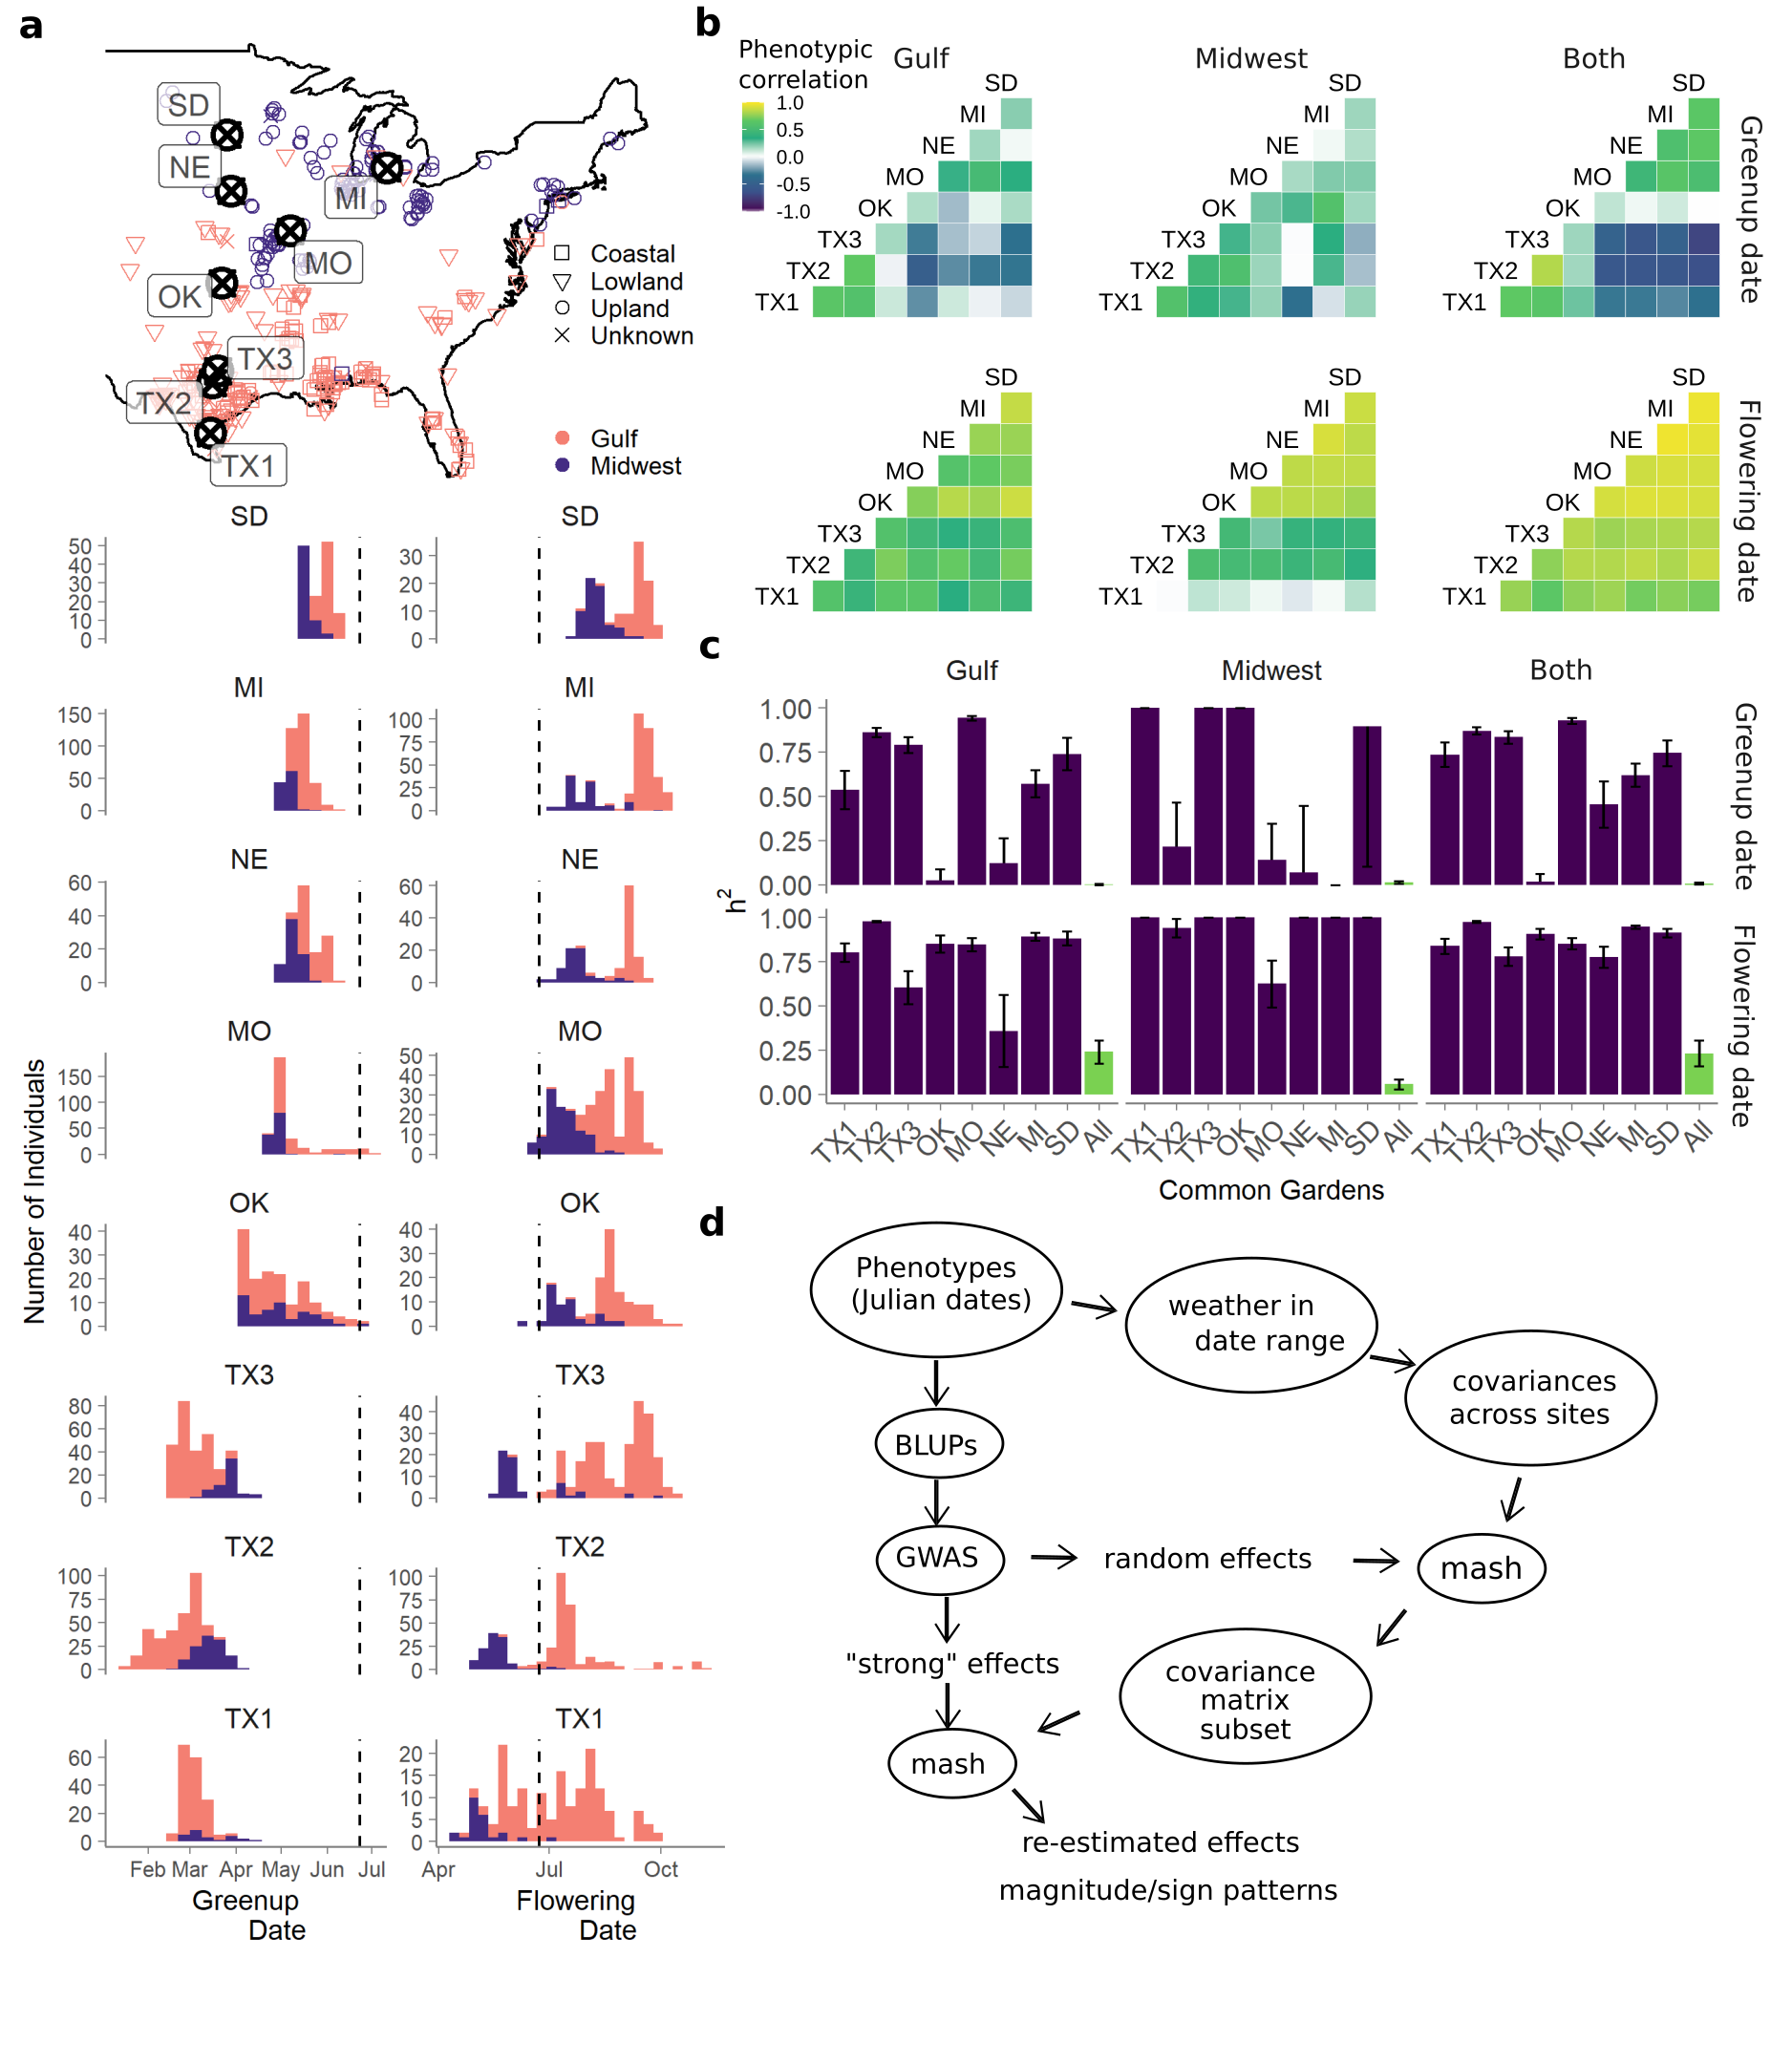
\includegraphics{images/Fig1_200dpi.png}

}

\caption{\label{fig-map}Characterization of green-up and flowering dates
from the switchgrass diversity panel. (a) Map and trait histograms of
green-up and flowering dates across two genetically distinct switchgrass
subpopulations and eight common gardens. Purple represents individuals
from the Midwest genetic subpopulation, and pink individuals from the
Gulf subpopulation. Vertical dashed lines indicate the summer solstice.
Common gardens are arranged in latitudinal order. (b) Phenotypic
correlations between clonal replicates planted at eight common gardens,
within and between two genetic subpopulations. (c) Narrow sense
heritability of green-up and flowering within single common gardens
(purple) and across all eight common gardens (green), within and between
two genetic subpopulations. (d) Flow diagram of the methods applied to
the green-up and flowering dates to jointly estimate SNP effects across
all sites. Mash was fit to SNP effect data and used to find covariance
matrices that improved the mash model likelihood using a large set of
randomly selected, relatively unlinked SNP effects; this model was
applied to a ``strong'' set of SNP effects with large effect sizes in
the univariate GWAS.}

\end{figure}%

\begin{figure}

\centering{

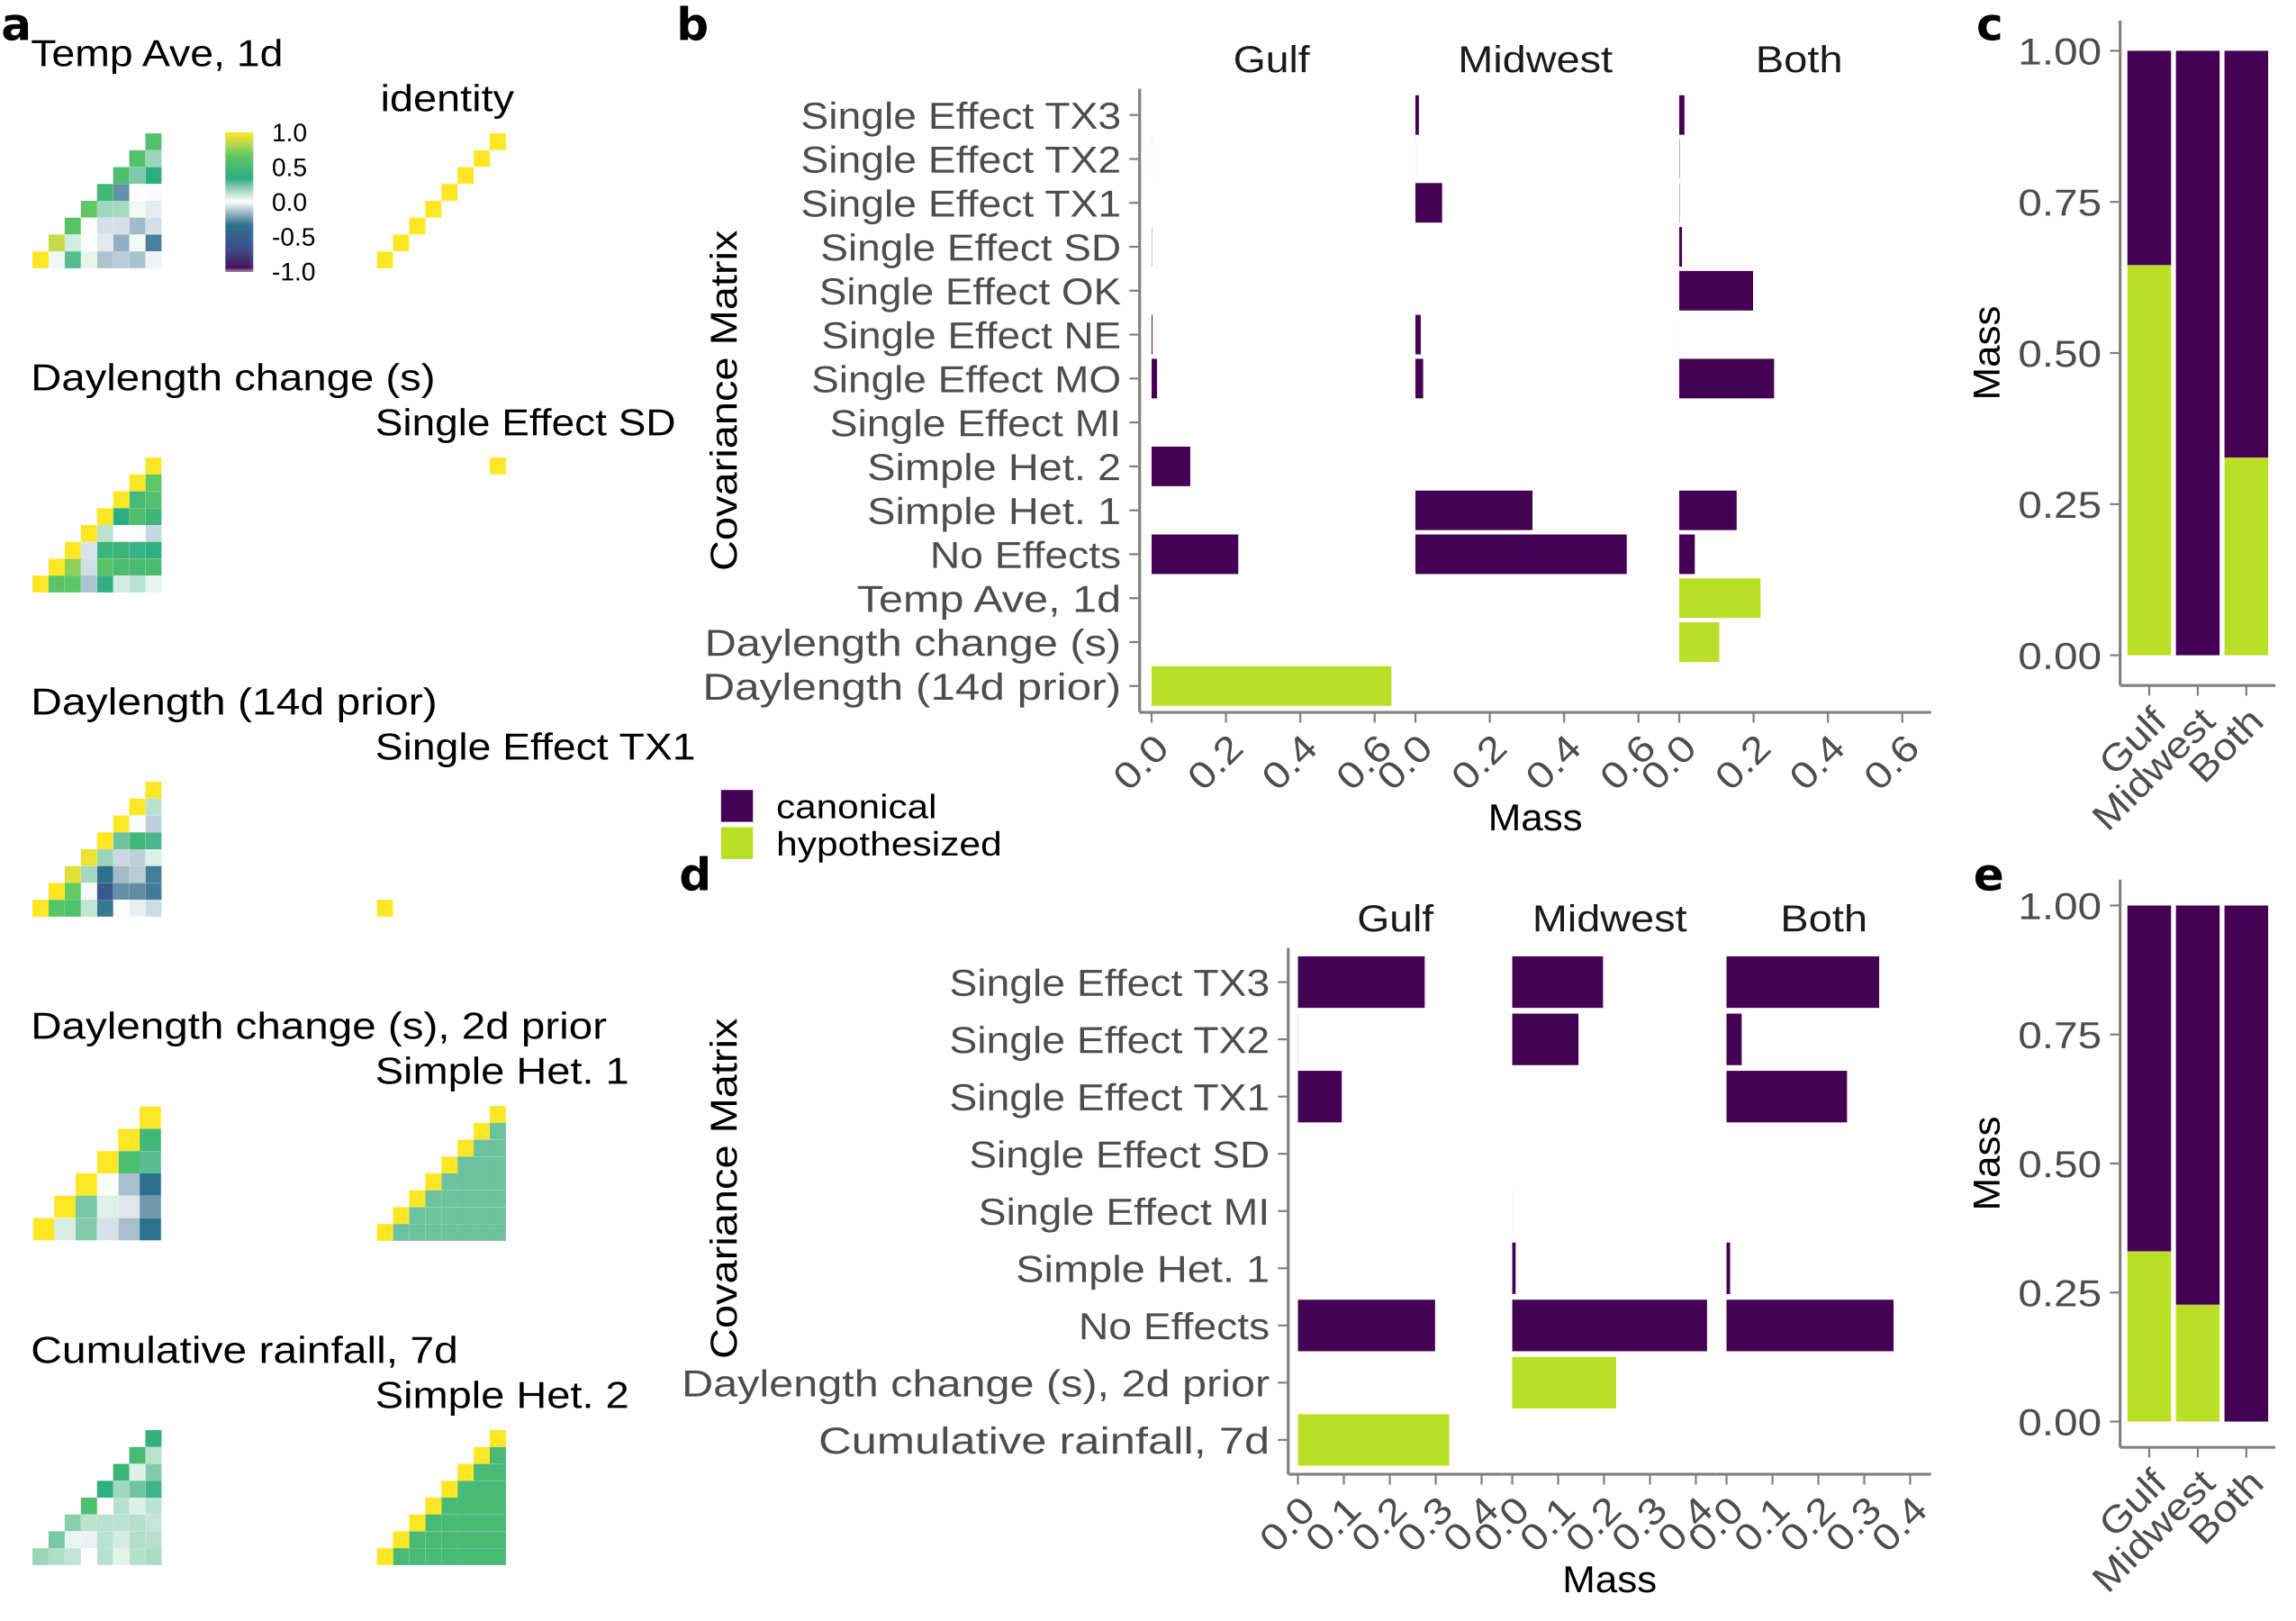
\includegraphics{images/Figure_2_Covariance_matrices_and_posterior_weights.png}

}

\caption{\label{fig-covar}Example hypothesis-driven covariance matrices
specified in mash and the posterior weights placed on all covariance
matrices. (a) Left column: Five example hypothesized covariance matrices
specified for the green-up date or flowering date phenotype; these
matrices were created from environment-specific correlations across
eight common gardens, and are described in Table XXX. Common gardens are
arranged in latitudinal order within the matrices. Right column: Five
example canonical covariance matrices. Canonical matrices (purple) have
simple interpretations, such as equal effects across all common gardens,
or effects specific to a single common garden. (b,d) Total posterior
weight placed on each covariance matrix type specified for (b) green-up
date and (d) flowering date mash models, within and between two genetic
subpopulations. Hypothesized covariance matrices (green). Covariance
matrices included in mash that had zero posterior weight in all three
mash runs on the genetic subpopulations, such as the identity matrix,
are not shown. (c,e) Total posterior weight placed on covariance
matrices that were hypothesized or canonical, for the (c) green-up date
phenotype and (e) flowering date phenotype.}

\end{figure}%

\begin{figure}

\centering{

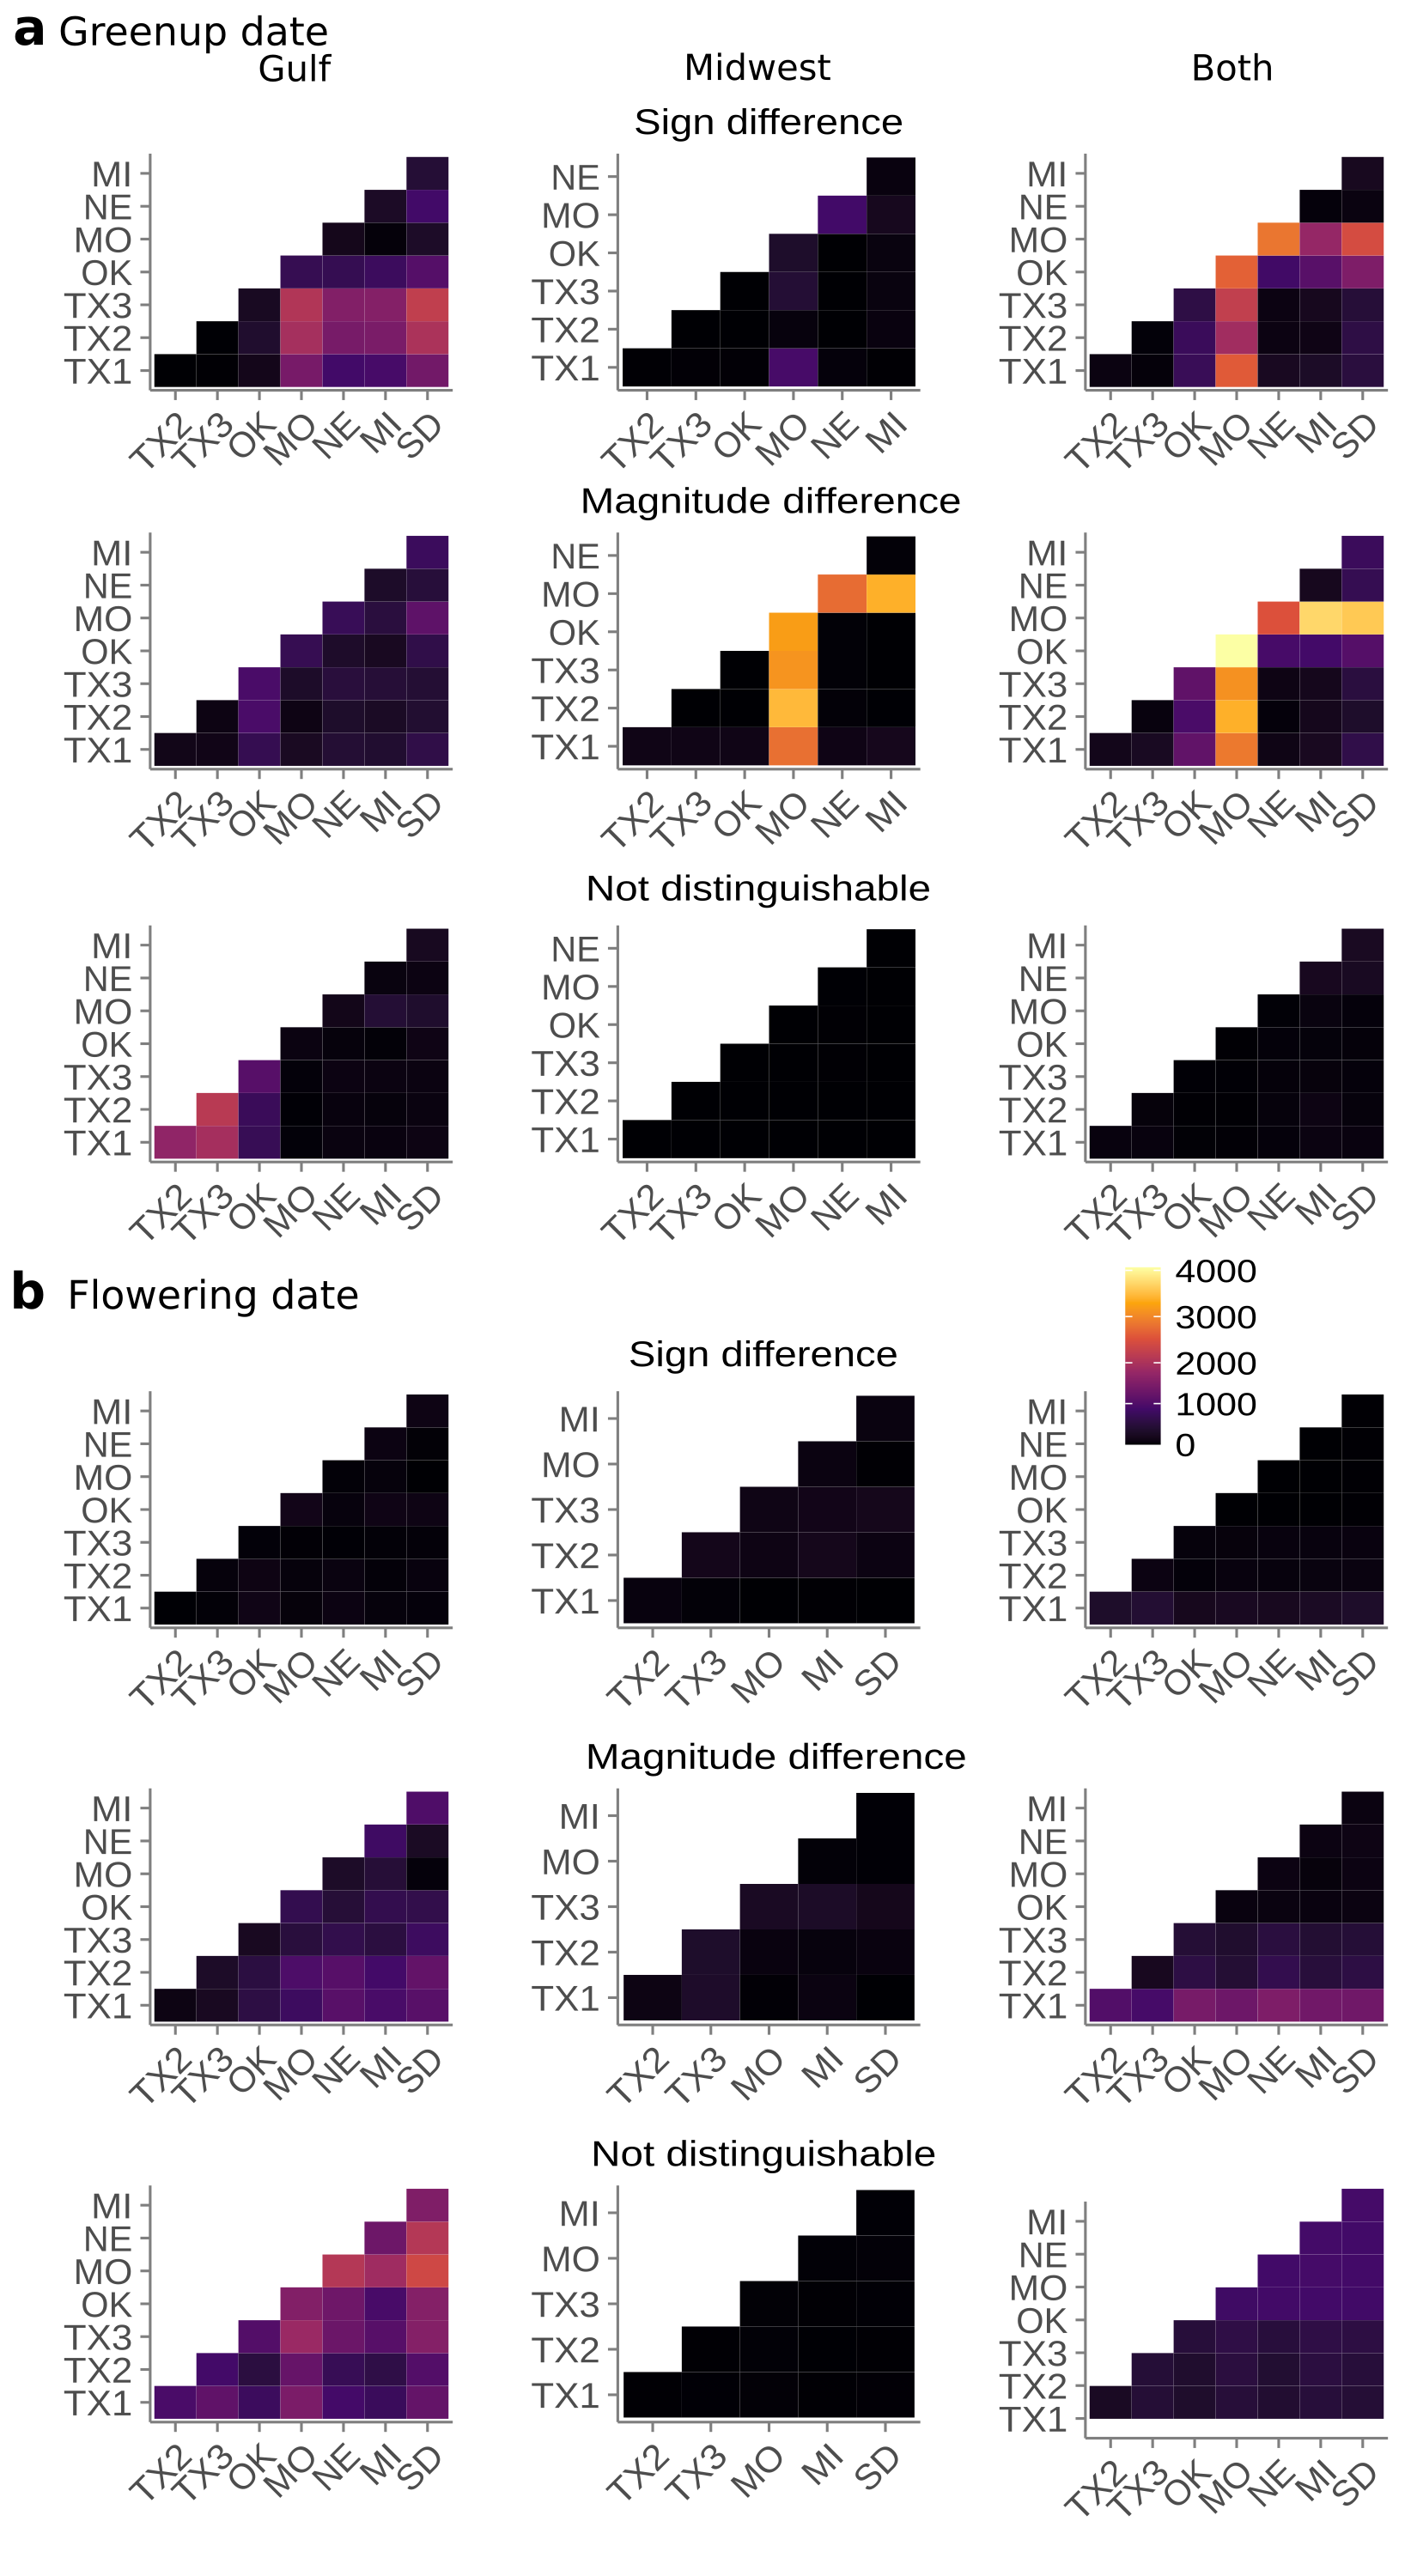
\includegraphics{images/Figure_3_Effect_Types_by_Site.png}

}

\caption{\label{fig-effects}Comparisons of pairs of jointly re-estimated
effects across eight gardens, for effects with lfsr \textless{} 0.05.
AHM is considering moving this figure to the supplement and
substantially simplifying the figure in the main text, perhaps just
showing total effects in Texas, the North, and maybe Oklahoma.
Essentially making Table 2 into a new, simplified figure. Effect
patterns for re-estimated SNP effects that are significant at pairs of
sites by the local false sign rate test (lfsr), for (a) greenup date and
(b) flowering date, within and between two genetic subpopulations.
Common gardens are arranged in latitudinal order along the x- and
y-axis. Effects in the first and fourth rows differ in sign at these
pairs of gardens (p \textless{} 0.05, lfsr). Effects in the second,
third, fifth and sixth rows are identical in sign (p \textless{} 0.05,
lfsr). Effects in the second and fifth rows additionally differ in
magnitude by a factor of \textgreater0.4, while effects in the third and
sixth row were not distinguishable by magnitude nor sign of the effect.}

\end{figure}%

\begin{figure}

\centering{

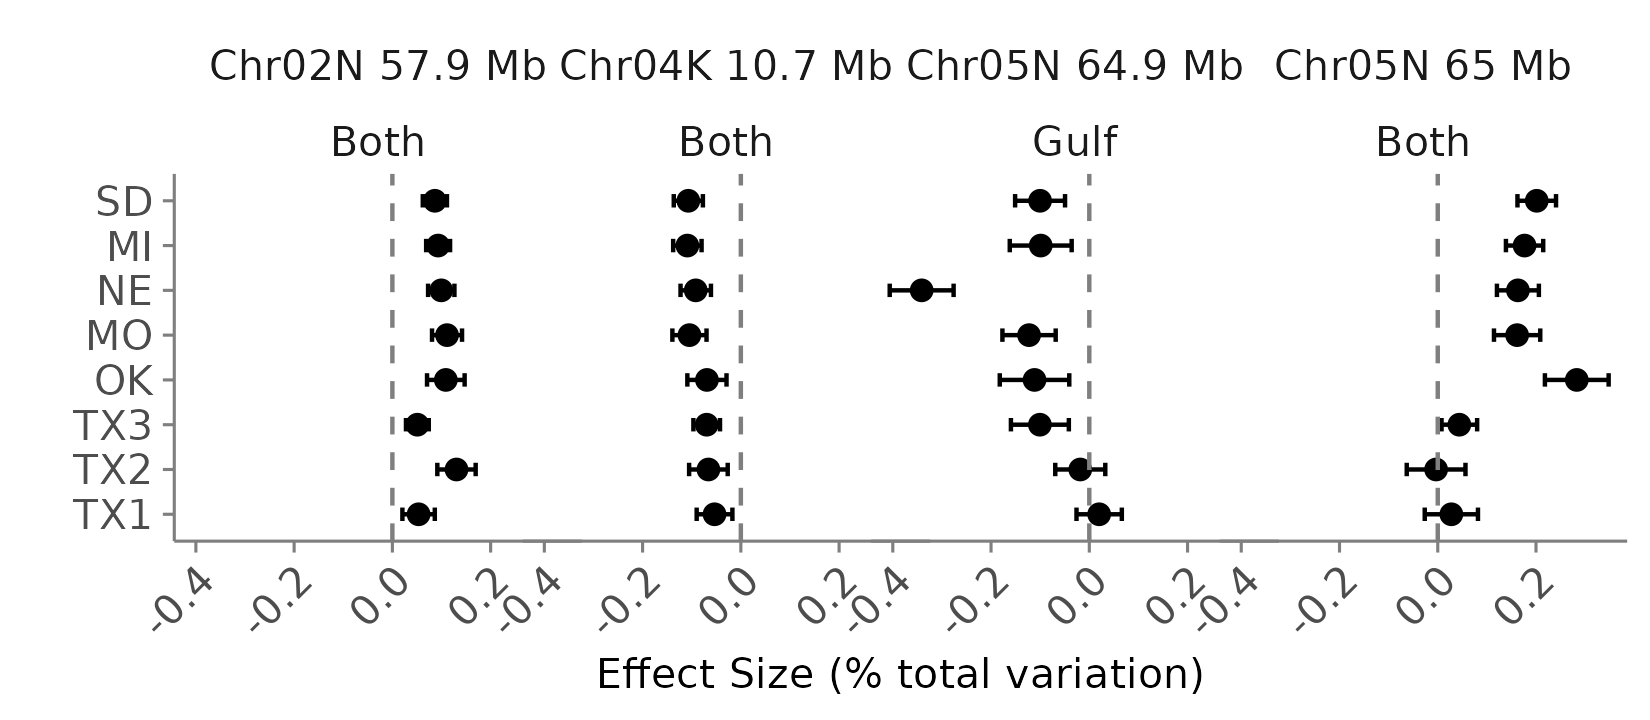
\includegraphics{images/Figure_4_mash_SNP_effects.png}

}

\caption{\label{fig-qtl}SNP effects for SNPs within QTL. AHM to re-make
this figure now LZ has re-run the QTL analysis, the assmption being the
re-analysis will not change the figure or the text much. The bigger
question for TEJ and AH is whether we want to keep this analysis in the
paper, what does it add?}

\end{figure}%

\section{Materials and Methods}\label{materials-and-methods}

Whenever possible, plant material will be shared upon request. Source
data and code to replicate these analyses are available at:
https://github.com/Alice-MacQueen/pvdiv-phenology-gxe.git. SNP data to
replicate these analyses are available from the UT dataverse at
https://doi.org/link.

\subsubsection{Genotype-by-environment effects on green-up and flowering
as functions of weather-based
cues}\label{genotype-by-environment-effects-on-green-up-and-flowering-as-functions-of-weather-based-cues}

In 2019, we scored two phenological events every two days in two mapping
populations of switchgrass, a diversity panel and a pseudo-F2 cross,
planted at eight common garden locations (32, 34, 37). We scored the
start of vegetative growth as the day of the year when 50\% of the
tiller area of the crown of the plant cut the previous year had green
growth. The start of reproductive growth, or flowering date, was the day
of the year when 50\% of the plant tillers had panicles undergoing
anthesis. We scored green-up and flowering as day of the year, then
linked these dates to multiple weather-based environmental factors
measured daily at each common garden (SI Appendix, Section S1, Table
S1).

The formation and resequencing of the diversity panel has been described
previously (32). The diversity panel contained 134 sequenced, clonally
propagated individuals from the Midwest genetic subpopulation, and 229
from the Gulf genetic subpopulation. To allow for the possibility that
different subpopulations had different strengths of connection between
our phenotypes and genotypes (38), we conducted three sets of genetic
analyses: on Gulf and Midwest genotypes separately, and on both
subpopulations together (`Both'). Analyses to determine narrow-sense
heritability (h\textsuperscript{2}) for green-up and flowering were done
using linear mixed models and followed (32). Details on these models can
be found in (SI Appendix, Section S3,S4).

\subsubsection{Mapping major patterns of genotype-by-environment effects
on green-up and
flowering}\label{mapping-major-patterns-of-genotype-by-environment-effects-on-green-up-and-flowering}

To evaluate the prevalence and kinds of covariance patterns of SNP
effects across our common gardens, we used multivariate adaptive
shrinkage (\emph{mash}) on SNP effect estimates from the diversity panel
(35). Mash is a statistical method that allows estimation and comparison
of many effects jointly across many different conditions; it improves on
previous methods by allowing multiple, arbitrary correlations in effect
sizes among conditions (SI Appendix, Section S5). To obtain SNP effect
estimates, we first conducted univariate genome-wide association at each
common garden for green-up and flowering date. We then analyzed SNP
effects for the top 19K relatively unlinked (r\textsuperscript{2}
\textless{} 0.2) SNPs per condition using mash, as in (32). Details on
these models can be found in (SI Appendix, Section S6).

We generated hypothesis-based covariance matrices derived from
correlations in environmental cues in the green-up or flowering date
windows for the three populations (SI Appendix, Table S1, Section S1).
These covariance matrices represent correlations between identical
genotypes drawn from a specific population at pairs of common gardens;
covariances near one mean that the population has a strong, positive
linear relationship in individual responses at that pair of gardens,
while covariances near zero mean that there is no relationship within
the population for individual responses at that pair of gardens. Mash
SNP effects will undergo strong shrinkage towards one another in the
first case, and little shrinkage in the second case. Mash also generates
data-driven covariance matrices corresponding to major patterns of SNP
effects present in the data. We generated six data-driven matrices per
mash run, five produced by singular value decomposition (SVD) of an
overall matrix.

Last, we characterized the overall patterns of antagonistic pleiotropy
in the set of SNPs where there was pairwise significance of effects at
pairs of gardens. To do this, we used the `get\_GxE' function of the
switchgrassGWAS R package. First, this determines the set of SNPs with
evidence of significant effects in both conditions for all pairs of
conditions using local false sign rates (lfsr) as the significance
criteria. Second, to determine antagonistic pleiotropy, this function
determines if effects significant in both conditions are of opposite
sign.

Using the lfsr rather than the local false discovery rate (lfdr) is a
critical change in our ability to detect antagonistic pleiotropy. The
lfdr, like other measures of FDR, focuses on if we have enough evidence
to reject the null hypothesis that an effect j is 0, or that there is a
significant effect. Previous studies of antagonistic pleiotropy
(e.g.~(37)) have used the lfdr or equivalent statistical tests to detect
antagonistic pleiotropy. These tests were conservative, in that they
required two non-zero effects of different signs, while tests for
differential sensitivity required only one non-zero effect. This
previous work recognized that this testing bias could lead to
undercounting occurrences of antagonistic pleiotropy (26, 27), and
sought to reduce it by permutation (28). However, using the lfsr to test
for antagonistic pleiotropy does not undercount occurrences of
antagonistic pleiotropy, as this statistic answers a fundamentally
different question. For each effect j, the lfsr\textsubscript{j} is
defined as the probability that we make an error in the sign of effect j
if we were forced to declare the effect positive or negative (36). Thus,
rather than asking ``Are these two effects different?'' - as we
reasonably expect two effects to be, even if this difference cannot be
measured - the local false sign rate answers a more meaningful question:
Can we be confident in the sign of this effect?

In addition, the get\_GxE function also sets an arbitrary threshold to
count an effect as changing in magnitude between environments, commonly
known as differential sensitivity or a change in amplitude of . For
differential sensitivity, this function determines if effects
significant in both conditions are of the same sign and of a magnitude
(not tested for significance) that differs by a factor of 0.4 or more.
The remaining effects that are significant in both conditions have the
same effect sign and similar effect magnitudes and we denote these
effects as having no GxE. The distinction between effects with different
magnitudes is arbitrary but useful to fully characterize how effects
vary across environments. and our use of the lfsr to determine
significance and our specification that SNP effects must be significant
in both conditions to be included means that our tests for antagonistic
pleiotropy carry an equal statistical burden to those measuring
differential sensitivity and effects without GxE.

\subsubsection{Confirmation of genotype-by-environment effects using an
independent mapping
population}\label{confirmation-of-genotype-by-environment-effects-using-an-independent-mapping-population}

To confirm candidate genomic regions and patterns of allelic effects
found in the diversity panel, we analyzed flowering in an outbred
pseudo-F2 cross between four individuals, two Midwest and two Gulf
individuals. The formation of this mapping population has been described
previously (34); additional details on QTL mapping can be found in SI
Appendix, Section S6. To be directly comparable to the diversity panel
data, only 2019 phenology data from the pseudo-F2 cross from the same
eight common garden sites were used. To compare our QTL enrichments of
significant mash associations to the null expectation, we used
permutation to choose 1000 sets of 23 genomic regions of the same size
randomly distributed throughout the genome, then calculated enrichments
of the mash 1\% tail in these random intervals.

\section{References}\label{references}

\bibsplit[2]

\phantomsection\label{refs}
\begin{CSLReferences}{0}{1}
\bibitem[\citeproctext]{ref-bauerle_photoperiodic_2012}
\CSLLeftMargin{1. }%
\CSLRightInline{W. L. Bauerle, \emph{et al.},
\href{https://doi.org/10.1073/pnas.1119131109}{Photoperiodic regulation
of the seasonal pattern of photosynthetic capacity and the implications
for carbon cycling}. \emph{Proceedings of the National Academy of
Sciences} \textbf{109}, 8612--8617 (2012).}

\bibitem[\citeproctext]{ref-andres2012genetic}
\CSLLeftMargin{2. }%
\CSLRightInline{F. Andrés, G. Coupland, The genetic basis of flowering
responses to seasonal cues. \emph{Nature Reviews Genetics} \textbf{13},
627--639 (2012).}

\bibitem[\citeproctext]{ref-korner2010phenology}
\CSLLeftMargin{3. }%
\CSLRightInline{C. Körner, D. Basler, Phenology under global warming.
\emph{Science} \textbf{327}, 1461--1462 (2010).}

\bibitem[\citeproctext]{ref-botero2015evolutionary}
\CSLLeftMargin{4. }%
\CSLRightInline{C. A. Botero, F. J. Weissing, J. Wright, D. R.
Rubenstein, Evolutionary tipping points in the capacity to adapt to
environmental change. \emph{Proceedings of the National Academy of
Sciences} \textbf{112}, 184--189 (2015).}

\bibitem[\citeproctext]{ref-blackman2013interacting}
\CSLLeftMargin{5. }%
\CSLRightInline{B. K. Blackman, Interacting duplications, fluctuating
selection, and convergence: The complex dynamics of flowering time
evolution during sunflower domestication. \emph{Journal of experimental
botany} \textbf{64}, 421--431 (2013).}

\bibitem[\citeproctext]{ref-henry2014transitions}
\CSLLeftMargin{6. }%
\CSLRightInline{L. P. Henry, R. H. Watson, B. K. Blackman, Transitions
in photoperiodic flowering are common and involve few loci in wild
sunflowers (helianthus; asteraceae). \emph{American Journal of Botany}
\textbf{101}, 1748--1758 (2014).}

\bibitem[\citeproctext]{ref-aagren2017adaptive}
\CSLLeftMargin{7. }%
\CSLRightInline{J. Ågren, C. G. Oakley, S. Lundemo, D. W. Schemske,
Adaptive divergence in flowering time among natural populations of
arabidopsis thaliana: Estimates of selection and QTL mapping.
\emph{Evolution} \textbf{71}, 550--564 (2017).}

\bibitem[\citeproctext]{ref-brachi2010linkage}
\CSLLeftMargin{8. }%
\CSLRightInline{B. Brachi, \emph{et al.}, Linkage and association
mapping of arabidopsis thaliana flowering time in nature. \emph{PLoS
genetics} \textbf{6}, e1000940 (2010).}

\bibitem[\citeproctext]{ref-dittmar2014flowering}
\CSLLeftMargin{9. }%
\CSLRightInline{E. L. Dittmar, C. G. Oakley, J. Ågren, D. W. Schemske,
Flowering time QTL in natural populations of arabidopsis thaliana and
implications for their adaptive value. \emph{Molecular ecology}
\textbf{23}, 4291--4303 (2014).}

\bibitem[\citeproctext]{ref-li2018genomic}
\CSLLeftMargin{10. }%
\CSLRightInline{X. Li, T. Guo, Q. Mu, X. Li, J. Yu, Genomic and
environmental determinants and their interplay underlying phenotypic
plasticity. \emph{Proceedings of the National Academy of Sciences}
\textbf{115}, 6679--6684 (2018).}

\bibitem[\citeproctext]{ref-romero2017study}
\CSLLeftMargin{11. }%
\CSLRightInline{J. A. Romero Navarro, \emph{et al.}, A study of allelic
diversity underlying flowering-time adaptation in maize landraces.
\emph{Nature genetics} \textbf{49}, 476--480 (2017).}

\bibitem[\citeproctext]{ref-wadgymar2017identifying}
\CSLLeftMargin{12. }%
\CSLRightInline{S. M. Wadgymar, \emph{et al.}, Identifying targets and
agents of selection: Innovative methods to evaluate the processes that
contribute to local adaptation. \emph{Methods in Ecology and Evolution}
\textbf{8}, 738--749 (2017).}

\bibitem[\citeproctext]{ref-blumel2015flowering}
\CSLLeftMargin{13. }%
\CSLRightInline{M. Blümel, N. Dally, C. Jung, Flowering time regulation
in crops---what did we learn from arabidopsis? \emph{Current opinion in
biotechnology} \textbf{32}, 121--129 (2015).}

\bibitem[\citeproctext]{ref-jung2009flowering}
\CSLLeftMargin{14. }%
\CSLRightInline{C. Jung, A. E. Müller, Flowering time control and
applications in plant breeding. \emph{Trends in plant science}
\textbf{14}, 563--573 (2009).}

\bibitem[\citeproctext]{ref-turner2005pseudo}
\CSLLeftMargin{15. }%
\CSLRightInline{A. Turner, J. Beales, S. Faure, R. P. Dunford, D. A.
Laurie, The pseudo-response regulator ppd-H1 provides adaptation to
photoperiod in barley. \emph{Science} \textbf{310}, 1031--1034 (2005).}

\bibitem[\citeproctext]{ref-faure2012mutation}
\CSLLeftMargin{16. }%
\CSLRightInline{S. Faure, \emph{et al.}, Mutation at the circadian clock
gene EARLY MATURITY 8 adapts domesticated barley (hordeum vulgare) to
short growing seasons. \emph{Proceedings of the National Academy of
Sciences} \textbf{109}, 8328--8333 (2012).}

\bibitem[\citeproctext]{ref-hung2012zmcct}
\CSLLeftMargin{17. }%
\CSLRightInline{H.-Y. Hung, \emph{et al.}, ZmCCT and the genetic basis
of day-length adaptation underlying the postdomestication spread of
maize. \emph{Proceedings of the National Academy of Sciences}
\textbf{109}, E1913--E1921 (2012).}

\bibitem[\citeproctext]{ref-zakhrabekova2012induced}
\CSLLeftMargin{18. }%
\CSLRightInline{S. Zakhrabekova, \emph{et al.}, Induced mutations in
circadian clock regulator mat-a facilitated short-season adaptation and
range extension in cultivated barley. \emph{Proceedings of the National
Academy of Sciences} \textbf{109}, 4326--4331 (2012).}

\bibitem[\citeproctext]{ref-yang2013oself3}
\CSLLeftMargin{19. }%
\CSLRightInline{Y. Yang, Q. Peng, G.-X. Chen, X.-H. Li, C.-Y. Wu, OsELF3
is involved in circadian clock regulation for promoting flowering under
long-day conditions in rice. \emph{Molecular Plant} \textbf{6}, 202--215
(2013).}

\bibitem[\citeproctext]{ref-pin2012multifaceted}
\CSLLeftMargin{20. }%
\CSLRightInline{P. Pin, O. Nilsson, The multifaceted roles of FLOWERING
LOCUS t in plant development. \emph{Plant, cell \& environment}
\textbf{35}, 1742--1755 (2012).}

\bibitem[\citeproctext]{ref-weller2019parallel}
\CSLLeftMargin{21. }%
\CSLRightInline{J. L. Weller, \emph{et al.}, Parallel origins of
photoperiod adaptation following dual domestications of common bean.
\emph{Journal of Experimental Botany} \textbf{70}, 1209--1219 (2019).}

\bibitem[\citeproctext]{ref-levene1953genetic}
\CSLLeftMargin{22. }%
\CSLRightInline{H. Levene, Genetic equilibrium when more than one
ecological niche is available. \emph{The American Naturalist}
\textbf{87}, 331--333 (1953).}

\bibitem[\citeproctext]{ref-felsenstein1976theoretical}
\CSLLeftMargin{23. }%
\CSLRightInline{J. Felsenstein, The theoretical population genetics of
variable selection and migration. \emph{Annual review of genetics}
\textbf{10}, 253--280 (1976).}

\bibitem[\citeproctext]{ref-kawecki2004conceptual}
\CSLLeftMargin{24. }%
\CSLRightInline{T. J. Kawecki, D. Ebert, Conceptual issues in local
adaptation. \emph{Ecology letters} \textbf{7}, 1225--1241 (2004).}

\bibitem[\citeproctext]{ref-hedrick1986genetic}
\CSLLeftMargin{25. }%
\CSLRightInline{P. W. Hedrick, Genetic polymorphism in heterogeneous
environments: A decade later. \emph{Annual review of ecology and
systematics} \textbf{17}, 535--566 (1986).}

\bibitem[\citeproctext]{ref-des2013genotype}
\CSLLeftMargin{26. }%
\CSLRightInline{D. L. Des Marais, K. M. Hernandez, T. E. Juenger,
Genotype-by-environment interaction and plasticity: Exploring genomic
responses of plants to the abiotic environment. \emph{Annual Review of
Ecology, Evolution, and Systematics} \textbf{44}, 5--29 (2013).}

\bibitem[\citeproctext]{ref-anderson2013genetic}
\CSLLeftMargin{27. }%
\CSLRightInline{J. T. Anderson, C.-R. Lee, C. A. Rushworth, R. I.
Colautti, T. Mitchell-Olds, Genetic trade-offs and conditional
neutrality contribute to local adaptation. \emph{Molecular ecology}
\textbf{22}, 699--708 (2013).}

\bibitem[\citeproctext]{ref-anderson2011evolutionary}
\CSLLeftMargin{28. }%
\CSLRightInline{J. T. Anderson, J. H. Willis, T. Mitchell-Olds,
Evolutionary genetics of plant adaptation. \emph{Trends in Genetics}
\textbf{27}, 258--266 (2011).}

\bibitem[\citeproctext]{ref-mitchell1997predicting}
\CSLLeftMargin{29. }%
\CSLRightInline{R. B. Mitchell, K. J. Moore, L. E. Moser, J. O. Fritz,
D. D. Redfearn, Predicting developmental morphology in switchgrass and
big bluestem. \emph{Agronomy Journal} \textbf{89}, 827--832 (1997).}

\bibitem[\citeproctext]{ref-parrish2005biology}
\CSLLeftMargin{30. }%
\CSLRightInline{D. J. Parrish, J. H. Fike, The biology and agronomy of
switchgrass for biofuels. \emph{BPTS} \textbf{24}, 423--459 (2005).}

\bibitem[\citeproctext]{ref-casler2004latitudinal}
\CSLLeftMargin{31. }%
\CSLRightInline{M. Casler, K. P. Vogel, C. Taliaferro, R. Wynia,
Latitudinal adaptation of switchgrass populations. \emph{Crop Science}
\textbf{44}, 293--303 (2004).}

\bibitem[\citeproctext]{ref-lovell2021genomic}
\CSLLeftMargin{32. }%
\CSLRightInline{J. T. Lovell, \emph{et al.}, Genomic mechanisms of
climate adaptation in polyploid bioenergy switchgrass. \emph{Nature}
\textbf{590}, 438--444 (2021).}

\bibitem[\citeproctext]{ref-porter1966analysis}
\CSLLeftMargin{33. }%
\CSLRightInline{C. L. Porter Jr, An analysis of variation between upland
and lowland switchgrass, panicum virgatum l., in central oklahoma.
\emph{Ecology} \textbf{47}, 980--992 (1966).}

\bibitem[\citeproctext]{ref-milano2016genetic}
\CSLLeftMargin{34. }%
\CSLRightInline{E. R. Milano, D. B. Lowry, T. E. Juenger, The genetic
basis of upland/lowland ecotype divergence in switchgrass (panicum
virgatum). \emph{G3: Genes, Genomes, Genetics} \textbf{6}, 3561--3570
(2016).}

\bibitem[\citeproctext]{ref-urbut2019flexible}
\CSLLeftMargin{35. }%
\CSLRightInline{S. M. Urbut, G. Wang, P. Carbonetto, M. Stephens,
Flexible statistical methods for estimating and testing effects in
genomic studies with multiple conditions. \emph{Nature genetics}
\textbf{51}, 187--195 (2019).}

\bibitem[\citeproctext]{ref-10.1093ux2fbiostatisticsux2fkxw041}
\CSLLeftMargin{36. }%
\CSLRightInline{M. Stephens,
\href{https://doi.org/10.1093/biostatistics/kxw041}{{False discovery
rates: a new deal}}. \emph{Biostatistics} \textbf{18}, 275--294 (2016).}

\bibitem[\citeproctext]{ref-savolainen2013ecological}
\CSLLeftMargin{37. }%
\CSLRightInline{O. Savolainen, M. Lascoux, J. Merilä, Ecological
genomics of local adaptation. \emph{Nature Reviews Genetics}
\textbf{14}, 807--820 (2013).}

\bibitem[\citeproctext]{ref-lowry2019qtl}
\CSLLeftMargin{38. }%
\CSLRightInline{D. B. Lowry, \emph{et al.}, QTL\(\times\) environment
interactions underlie adaptive divergence in switchgrass across a large
latitudinal gradient. \emph{Proceedings of the National Academy of
Sciences} \textbf{116}, 12933--12941 (2019).}

\end{CSLReferences}

\acknow{We thank the Brackenridge Field laboratory, the Ladybird Johnson
Wildflower Center, and the Juenger laboratory for support with plant
care and propagation. This material is based upon work supported in part
by the Great Lakes Bioenergy Research Center, U.S. Department of Energy,
Office of Science, Office of Biological and Environmental Research under
Award Numbers DE-SC0018409 and DE-FC02-07ER64494, the US Department of
Energy Awards DESC0014156 to T.E.J., DE-SC0017883 to D.B.L, National
Science Foundation PGRP Awards IOS0922457 and IOS1444533 to T.E.J, and
the Long-term Ecological Research Program (DEB 1832042) at the Kellogg
Biological Station.}

\showacknow{} % Display the acknowledgments section


\end{document}
